\documentclass[]{article}
\usepackage{lmodern}
\usepackage{amssymb,amsmath}
\usepackage{ifxetex,ifluatex}
\usepackage{fixltx2e} % provides \textsubscript
\ifnum 0\ifxetex 1\fi\ifluatex 1\fi=0 % if pdftex
  \usepackage[T1]{fontenc}
  \usepackage[utf8]{inputenc}
\else % if luatex or xelatex
  \ifxetex
    \usepackage{mathspec}
  \else
    \usepackage{fontspec}
  \fi
  \defaultfontfeatures{Ligatures=TeX,Scale=MatchLowercase}
\fi
% use upquote if available, for straight quotes in verbatim environments
\IfFileExists{upquote.sty}{\usepackage{upquote}}{}
% use microtype if available
\IfFileExists{microtype.sty}{%
\usepackage{microtype}
\UseMicrotypeSet[protrusion]{basicmath} % disable protrusion for tt fonts
}{}
\usepackage[margin=1in]{geometry}
\usepackage{hyperref}
\hypersetup{unicode=true,
            pdftitle={Ocular Sampling in Google Earth Engine},
            pdfauthor={Tim Mayer \& Dan Carver},
            pdfborder={0 0 0},
            breaklinks=true}
\urlstyle{same}  % don't use monospace font for urls
\usepackage{color}
\usepackage{fancyvrb}
\newcommand{\VerbBar}{|}
\newcommand{\VERB}{\Verb[commandchars=\\\{\}]}
\DefineVerbatimEnvironment{Highlighting}{Verbatim}{commandchars=\\\{\}}
% Add ',fontsize=\small' for more characters per line
\usepackage{framed}
\definecolor{shadecolor}{RGB}{248,248,248}
\newenvironment{Shaded}{\begin{snugshade}}{\end{snugshade}}
\newcommand{\KeywordTok}[1]{\textcolor[rgb]{0.13,0.29,0.53}{\textbf{#1}}}
\newcommand{\DataTypeTok}[1]{\textcolor[rgb]{0.13,0.29,0.53}{#1}}
\newcommand{\DecValTok}[1]{\textcolor[rgb]{0.00,0.00,0.81}{#1}}
\newcommand{\BaseNTok}[1]{\textcolor[rgb]{0.00,0.00,0.81}{#1}}
\newcommand{\FloatTok}[1]{\textcolor[rgb]{0.00,0.00,0.81}{#1}}
\newcommand{\ConstantTok}[1]{\textcolor[rgb]{0.00,0.00,0.00}{#1}}
\newcommand{\CharTok}[1]{\textcolor[rgb]{0.31,0.60,0.02}{#1}}
\newcommand{\SpecialCharTok}[1]{\textcolor[rgb]{0.00,0.00,0.00}{#1}}
\newcommand{\StringTok}[1]{\textcolor[rgb]{0.31,0.60,0.02}{#1}}
\newcommand{\VerbatimStringTok}[1]{\textcolor[rgb]{0.31,0.60,0.02}{#1}}
\newcommand{\SpecialStringTok}[1]{\textcolor[rgb]{0.31,0.60,0.02}{#1}}
\newcommand{\ImportTok}[1]{#1}
\newcommand{\CommentTok}[1]{\textcolor[rgb]{0.56,0.35,0.01}{\textit{#1}}}
\newcommand{\DocumentationTok}[1]{\textcolor[rgb]{0.56,0.35,0.01}{\textbf{\textit{#1}}}}
\newcommand{\AnnotationTok}[1]{\textcolor[rgb]{0.56,0.35,0.01}{\textbf{\textit{#1}}}}
\newcommand{\CommentVarTok}[1]{\textcolor[rgb]{0.56,0.35,0.01}{\textbf{\textit{#1}}}}
\newcommand{\OtherTok}[1]{\textcolor[rgb]{0.56,0.35,0.01}{#1}}
\newcommand{\FunctionTok}[1]{\textcolor[rgb]{0.00,0.00,0.00}{#1}}
\newcommand{\VariableTok}[1]{\textcolor[rgb]{0.00,0.00,0.00}{#1}}
\newcommand{\ControlFlowTok}[1]{\textcolor[rgb]{0.13,0.29,0.53}{\textbf{#1}}}
\newcommand{\OperatorTok}[1]{\textcolor[rgb]{0.81,0.36,0.00}{\textbf{#1}}}
\newcommand{\BuiltInTok}[1]{#1}
\newcommand{\ExtensionTok}[1]{#1}
\newcommand{\PreprocessorTok}[1]{\textcolor[rgb]{0.56,0.35,0.01}{\textit{#1}}}
\newcommand{\AttributeTok}[1]{\textcolor[rgb]{0.77,0.63,0.00}{#1}}
\newcommand{\RegionMarkerTok}[1]{#1}
\newcommand{\InformationTok}[1]{\textcolor[rgb]{0.56,0.35,0.01}{\textbf{\textit{#1}}}}
\newcommand{\WarningTok}[1]{\textcolor[rgb]{0.56,0.35,0.01}{\textbf{\textit{#1}}}}
\newcommand{\AlertTok}[1]{\textcolor[rgb]{0.94,0.16,0.16}{#1}}
\newcommand{\ErrorTok}[1]{\textcolor[rgb]{0.64,0.00,0.00}{\textbf{#1}}}
\newcommand{\NormalTok}[1]{#1}
\usepackage{graphicx,grffile}
\makeatletter
\def\maxwidth{\ifdim\Gin@nat@width>\linewidth\linewidth\else\Gin@nat@width\fi}
\def\maxheight{\ifdim\Gin@nat@height>\textheight\textheight\else\Gin@nat@height\fi}
\makeatother
% Scale images if necessary, so that they will not overflow the page
% margins by default, and it is still possible to overwrite the defaults
% using explicit options in \includegraphics[width, height, ...]{}
\setkeys{Gin}{width=\maxwidth,height=\maxheight,keepaspectratio}
\IfFileExists{parskip.sty}{%
\usepackage{parskip}
}{% else
\setlength{\parindent}{0pt}
\setlength{\parskip}{6pt plus 2pt minus 1pt}
}
\setlength{\emergencystretch}{3em}  % prevent overfull lines
\providecommand{\tightlist}{%
  \setlength{\itemsep}{0pt}\setlength{\parskip}{0pt}}
\setcounter{secnumdepth}{0}
% Redefines (sub)paragraphs to behave more like sections
\ifx\paragraph\undefined\else
\let\oldparagraph\paragraph
\renewcommand{\paragraph}[1]{\oldparagraph{#1}\mbox{}}
\fi
\ifx\subparagraph\undefined\else
\let\oldsubparagraph\subparagraph
\renewcommand{\subparagraph}[1]{\oldsubparagraph{#1}\mbox{}}
\fi

%%% Use protect on footnotes to avoid problems with footnotes in titles
\let\rmarkdownfootnote\footnote%
\def\footnote{\protect\rmarkdownfootnote}

%%% Change title format to be more compact
\usepackage{titling}

% Create subtitle command for use in maketitle
\newcommand{\subtitle}[1]{
  \posttitle{
    \begin{center}\large#1\end{center}
    }
}

\setlength{\droptitle}{-2em}

  \title{Ocular Sampling in Google Earth Engine}
    \pretitle{\vspace{\droptitle}\centering\huge}
  \posttitle{\par}
    \author{Tim Mayer \& Dan Carver}
    \preauthor{\centering\large\emph}
  \postauthor{\par}
      \predate{\centering\large\emph}
  \postdate{\par}
    \date{updated: 01/11/2019}


\begin{document}
\maketitle

{
\setcounter{tocdepth}{2}
\tableofcontents
}
\section{Google Earth Engine}\label{google-earth-engine}

This resource has changed our methods for working with remotely sensed
data. Google Earth Engine is a web based analysis platform that provides
access to large libraries of geospatial data. For the most part the
available data is raster based. What is nice about the resource it that
it takes away the downloading and preprocessing aspects of the working
with these datasets. This allows you to move into asking your question
and develop methodology very rapidly. GEE does require registration to a
google account. You can sign up and read more at this
link:\href{https://earthengine.google.com/}{sign up}

\subsection{Goal}\label{goal}

In this document we will show how to use high resolution NAIP imagery
and NLCD to visually sample for a specific land cover class. This is a
method that allows you to add to existing presence and absence
locations.

\subsection{Background on datasets}\label{background-on-datasets}

NLCD:The National Land Cover Database is a 30-m Landsat-based land cover
database spanning 4 epochs (1992, 2001, 2006 and 2011). 1992 data are
primarily based on unsupervised classification of Landsat data, while
the rest of the images rely on the imperviousness data layer for the
urban classes and on a decision-tree classification for the rest.

NAIP:The National Agriculture Imagery Program acquires aerial imagery
during the agricultural growing seasons in the continental US. NAIP
projects are contracted each year based upon available funding and the
FSA imagery acquisition cycle. Beginning in 2003, NAIP was acquired on a
5-year cycle. 2008 was a transition year, and a three-year cycle began
in 2009. NAIP imagery is acquired at a one-meter ground sample distance
(GSD) with a horizontal accuracy that matches within six meters of
photo-identifiable ground control points, which are used during image
inspection. Depending on the given location and time frame, NAIP imagery
is collected in 4 bands, blue, green, red, and near infrared. The near
infrared band is helpful in distinguishing between different types of
vegetation.

\subsection{Setting up Sampling
Interface}\label{setting-up-sampling-interface}

In this example we will sample Quaking Aspen (Populus tremuloides) in
the Grand Mesa region of CO for 2015.

We will load both true color and false color NAIP imagery to allow for
the best distinction as well as NLCD to aid with sampling.

\subsection{Define Region of Interest}\label{define-region-of-interest}

Creating geometries in earth engine is as simple as pressing the
geometry button.

\begin{figure}
\centering
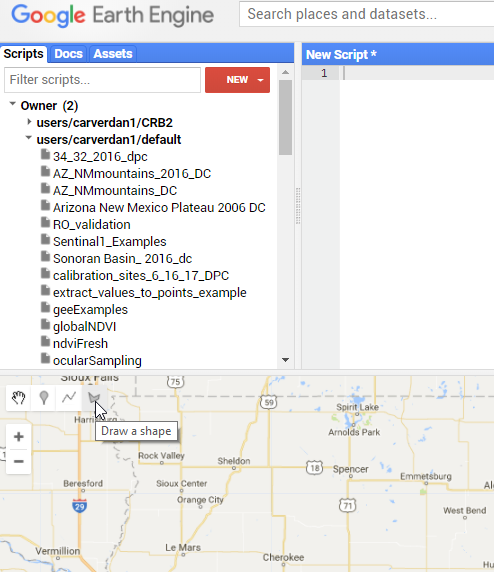
\includegraphics{drawPolygon.png}
\caption{geometry button}
\end{figure}

 Click on locations on the map that you want as you region of interest

\begin{figure}
\centering
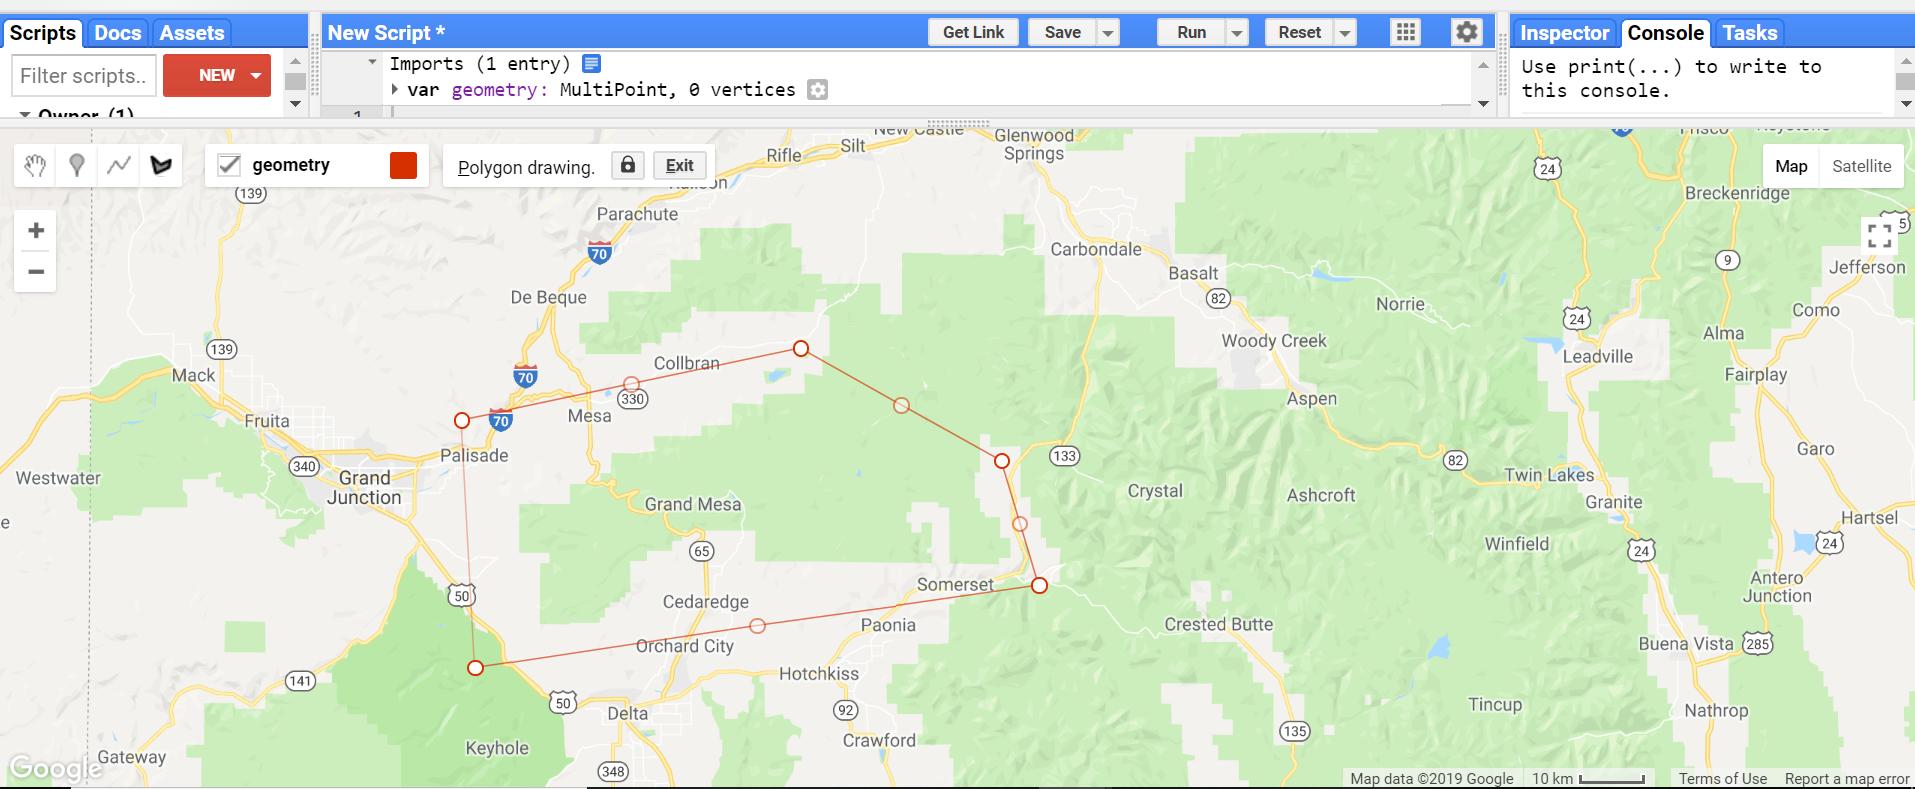
\includegraphics{Make_Geometry_ScreenShot1.png}
\caption{region of interest}
\end{figure}

 Once you complete the geometry feature by placing a point on the
starting location, a new feature will appear in your text editor.
Leaving this named geometry is fine for now.

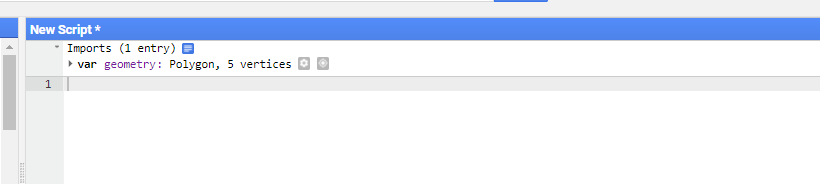
\includegraphics{geometryImport.png}

\subsection{Loading In NAIP Imagery}\label{loading-in-naip-imagery}

We started with the plan to sample from the year 2015. However since we
used GEE we gave ourselves a few more options. The code below allows you
to call in the imagery and filter it for both 2015 and 2016. This is
helpfull because NAIP is not collected every year.

\begin{Shaded}
\begin{Highlighting}[]
\CommentTok{// call in NAIP imagery as an image collection}
\KeywordTok{var}\NormalTok{ NAIP }\OperatorTok{=} \VariableTok{ee}\NormalTok{.}\AttributeTok{ImageCollection}\NormalTok{(}\StringTok{"USDA/NAIP/DOQQ"}\NormalTok{)}

\CommentTok{// filter the data based on date and area for 2015}
\KeywordTok{var}\NormalTok{ naip2015 }\OperatorTok{=}\NormalTok{ NAIP}
\NormalTok{  .}\AttributeTok{filterBounds}\NormalTok{(geometry)}
\NormalTok{  .}\AttributeTok{filterDate}\NormalTok{(}\StringTok{"2015-01-01"}\OperatorTok{,} \StringTok{"2015-12-31"}\NormalTok{)}
\CommentTok{// filter the data based on date and area for 2016}
\KeywordTok{var}\NormalTok{ naip2016 }\OperatorTok{=}\NormalTok{ NAIP}
\NormalTok{  .}\AttributeTok{filterBounds}\NormalTok{(geometry)}
\NormalTok{  .}\AttributeTok{filterDate}\NormalTok{(}\StringTok{"2016-01-01"}\OperatorTok{,} \StringTok{"2016-12-31"}\NormalTok{)}
\end{Highlighting}
\end{Shaded}

\subsection{Adding images to the map}\label{adding-images-to-the-map}

Now that we've loaded the imagery we want to visulize it on the map.
NAIP imagery is collected as a series of images. Therefore we need to
create a multispectral image by defines what bands we want to use. We do
this by setting visulization parameters. Once those are defined we can
add the images to the map. In this case we're going to add true color
and color composites for both 2015 and 2016 because we don't really know
when the imagery was captured for your area of interest.

\begin{Shaded}
\begin{Highlighting}[]

\CommentTok{//define viewing parameters for multi band images}
\KeywordTok{var}\NormalTok{ visParams }\OperatorTok{=} \OperatorTok{\{}\DataTypeTok{bands}\OperatorTok{:}\NormalTok{[}\StringTok{'N'}\OperatorTok{,} \StringTok{'R'}\OperatorTok{,} \StringTok{'G'}\NormalTok{]}\OperatorTok{\}}
\KeywordTok{var}\NormalTok{ visParams1 }\OperatorTok{=} \OperatorTok{\{}\DataTypeTok{bands}\OperatorTok{:}\NormalTok{[}\StringTok{'R'}\OperatorTok{,} \StringTok{'G'}\OperatorTok{,} \StringTok{'B'}\NormalTok{]}\OperatorTok{\}}

\CommentTok{// add 2015 imagery to the map with false color and true color composites}
\VariableTok{Map}\NormalTok{.}\AttributeTok{addLayer}\NormalTok{(naip2015}\OperatorTok{,}\NormalTok{visParams}\OperatorTok{,}\StringTok{"2015_false"}\OperatorTok{,}\KeywordTok{false}\NormalTok{ )}
\VariableTok{Map}\NormalTok{.}\AttributeTok{addLayer}\NormalTok{(naip2015}\OperatorTok{,}\NormalTok{visParams1}\OperatorTok{,}\StringTok{"2015_true"}\OperatorTok{,}\KeywordTok{false}\NormalTok{ )}

\CommentTok{// add 2016 imagery to the map with false color and true color composites}
\VariableTok{Map}\NormalTok{.}\AttributeTok{addLayer}\NormalTok{(naip2016}\OperatorTok{,}\NormalTok{visParams}\OperatorTok{,}\StringTok{"2016_false"}\OperatorTok{,}\KeywordTok{false}\NormalTok{ )}
\VariableTok{Map}\NormalTok{.}\AttributeTok{addLayer}\NormalTok{(naip2016}\OperatorTok{,}\NormalTok{visParams1}\OperatorTok{,}\StringTok{"2016_true"}\OperatorTok{,}\KeywordTok{false}\NormalTok{ )}
\end{Highlighting}
\end{Shaded}

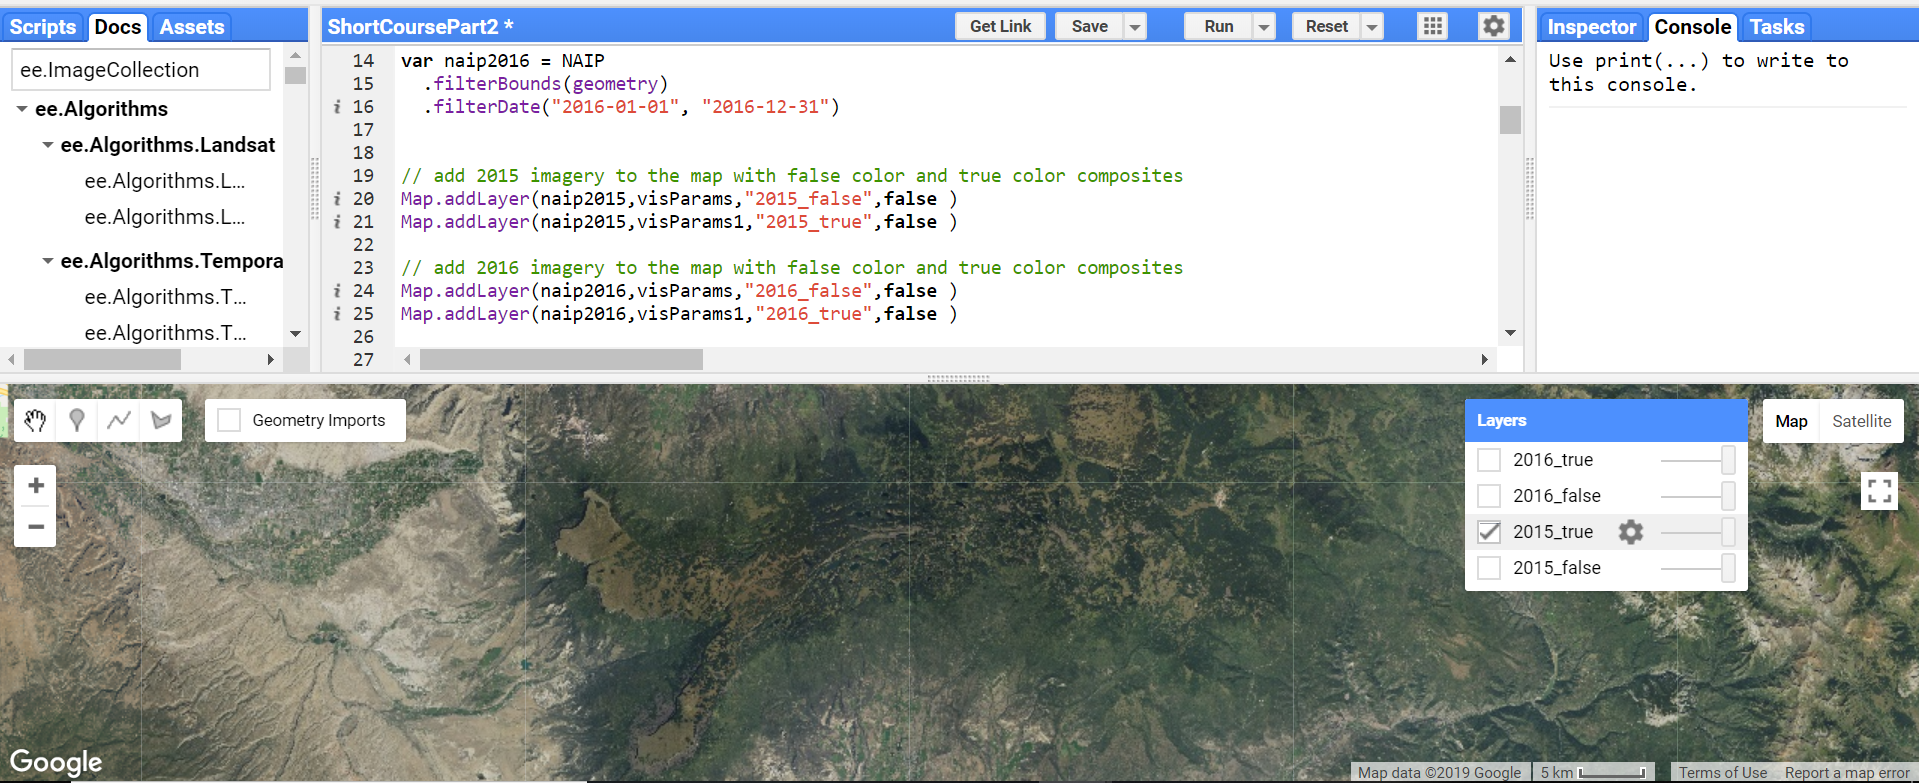
\includegraphics{True_Color_ScreenShot1.png}

\subsection{Loading In NLCD Imagery}\label{loading-in-nlcd-imagery}

Now we will also add the NLCD layer to give you a better reference
regarding landcover, which can be assit with sampling in latter steps.

\begin{Shaded}
\begin{Highlighting}[]

\CommentTok{//add National Land Cover Database (NLCD) with color palette}
\KeywordTok{var}\NormalTok{ dataset }\OperatorTok{=} \VariableTok{ee}\NormalTok{.}\AttributeTok{ImageCollection}\NormalTok{(}\StringTok{'USGS/NLCD'}\NormalTok{)}
\CommentTok{////////comment out this line of code to unclip the NLCD layer from the geometry//////////}
\NormalTok{  .}\AttributeTok{map}\NormalTok{(}\KeywordTok{function}\NormalTok{(image) }\OperatorTok{\{} \ControlFlowTok{return} \VariableTok{image}\NormalTok{.}\AttributeTok{clip}\NormalTok{(geometry)}\OperatorTok{;} \OperatorTok{\}}\NormalTok{)}\OperatorTok{;}
\CommentTok{//}
\KeywordTok{var}\NormalTok{ landcover }\OperatorTok{=} \VariableTok{dataset}\NormalTok{.}\AttributeTok{select}\NormalTok{(}\StringTok{'landcover'}\NormalTok{)}
\end{Highlighting}
\end{Shaded}

\subsection{Visualize the NLCD layer using a color
pallete}\label{visualize-the-nlcd-layer-using-a-color-pallete}

Notice the color codes. More information about these colors and
subsequent classes can be found by searching NLCD in Googel Earth
Engines search window.

\begin{Shaded}
\begin{Highlighting}[]

\KeywordTok{var}\NormalTok{ landcover }\OperatorTok{=} \VariableTok{dataset}\NormalTok{.}\AttributeTok{select}\NormalTok{(}\StringTok{'landcover'}\NormalTok{)}
\CommentTok{//}
\KeywordTok{var}\NormalTok{ landcoverVis }\OperatorTok{=} \OperatorTok{\{}
  \DataTypeTok{min}\OperatorTok{:} \FloatTok{11.0}\OperatorTok{,}
  \DataTypeTok{max}\OperatorTok{:} \FloatTok{95.0}\OperatorTok{,}
  \DataTypeTok{palette}\OperatorTok{:}\NormalTok{ [}
    \StringTok{'5475A8'}\OperatorTok{,} \StringTok{'ffffff'}\OperatorTok{,} \StringTok{'E8D1D1'}\OperatorTok{,} \StringTok{'E29E8C'}\OperatorTok{,} \StringTok{'ff0000'}\OperatorTok{,} \StringTok{'B50000'}\OperatorTok{,} \StringTok{'D2CDC0'}\OperatorTok{,}
    \StringTok{'85C77E'}\OperatorTok{,} \StringTok{'38814E'}\OperatorTok{,} \StringTok{'D4E7B0'}\OperatorTok{,} \StringTok{'AF963C'}\OperatorTok{,} \StringTok{'DCCA8F'}\OperatorTok{,} \StringTok{'FDE9AA'}\OperatorTok{,} \StringTok{'D1D182'}\OperatorTok{,}
    \StringTok{'A3CC51'}\OperatorTok{,} \StringTok{'82BA9E'}\OperatorTok{,} \StringTok{'FBF65D'}\OperatorTok{,} \StringTok{'CA9146'}\OperatorTok{,} \StringTok{'C8E6F8'}\OperatorTok{,} \StringTok{'64B3D5'}
\NormalTok{  ]}\OperatorTok{,}
\OperatorTok{\};}
\end{Highlighting}
\end{Shaded}

Now lets add this layer to the map and center the image.

\begin{Shaded}
\begin{Highlighting}[]

\VariableTok{Map}\NormalTok{.}\AttributeTok{addLayer}\NormalTok{(landcover}\OperatorTok{,}\NormalTok{ landcoverVis}\OperatorTok{,} \StringTok{'National Land Cover Database (NLCD)'}\OperatorTok{,}\KeywordTok{false}\NormalTok{)}\OperatorTok{;}
\VariableTok{Map}\NormalTok{.}\AttributeTok{setCenter}\NormalTok{(}\OperatorTok{-}\FloatTok{107.993660}\OperatorTok{,} \FloatTok{39.007467}\OperatorTok{,} \DecValTok{10}\NormalTok{)}\OperatorTok{;}
\end{Highlighting}
\end{Shaded}

\begin{figure}
\centering
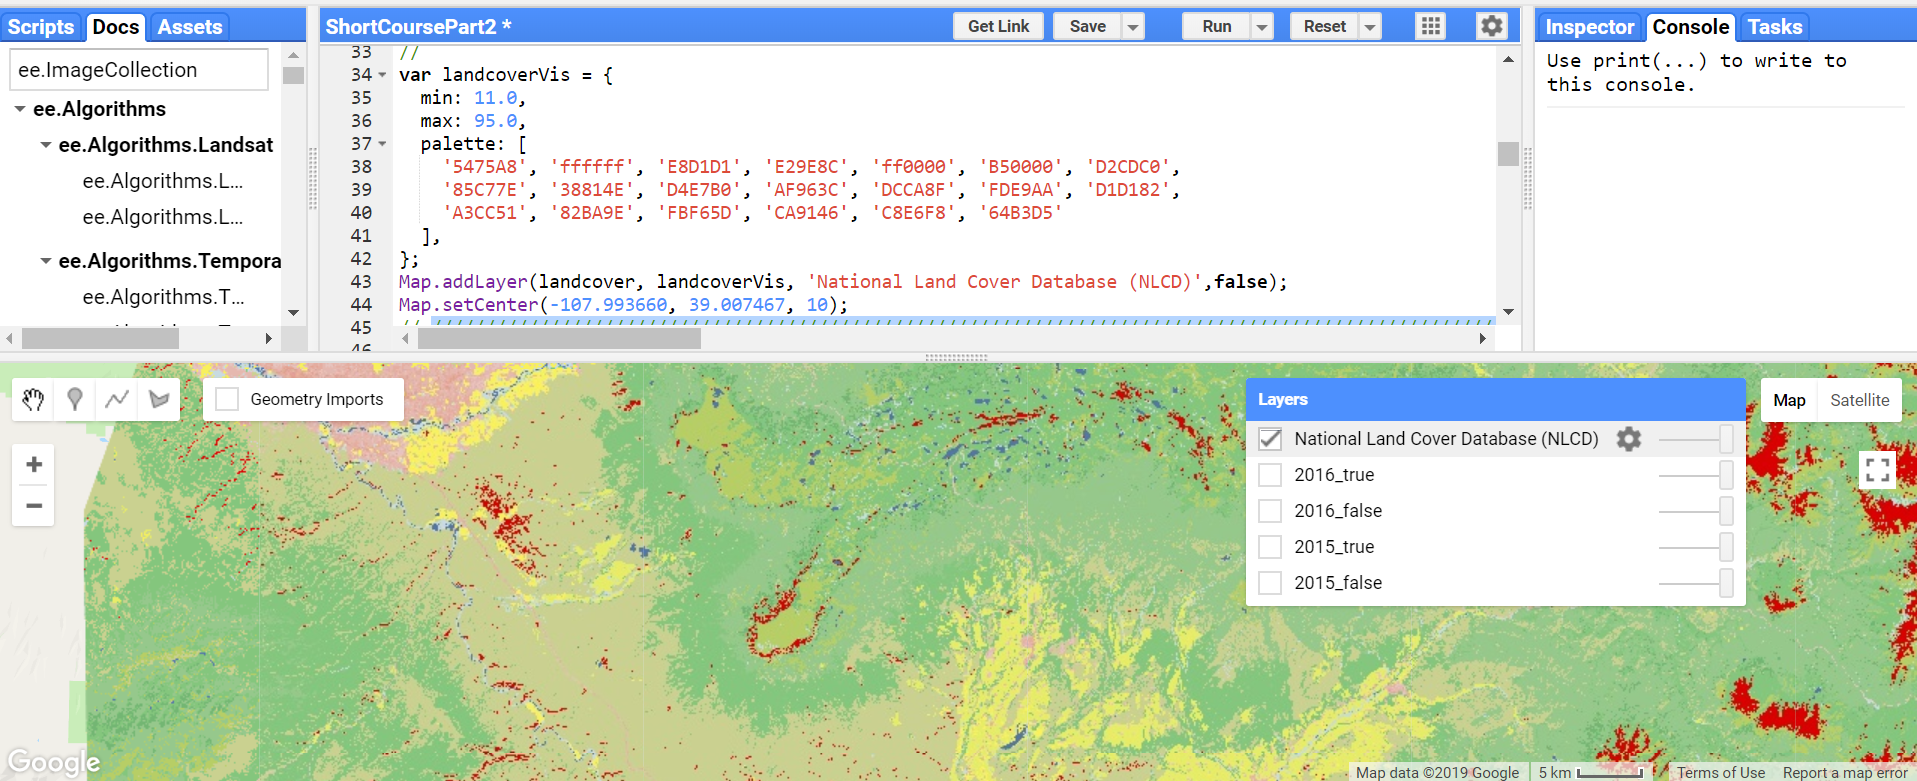
\includegraphics{NLCD_ScreenShot.png}
\caption{NLCD}
\end{figure}

\subsection{Add a legend to the NLCD
layer}\label{add-a-legend-to-the-nlcd-layer}

This additional segement of code definign the legend of the NLCD can
help with investigating different classes during sampling.

\begin{Shaded}
\begin{Highlighting}[]

\CommentTok{///////////////////////////////////////////////////////////////////////////////////////////////////}
\CommentTok{/////////////////////////////////////////////////Legend////////////////////////////////////////////}
\CommentTok{///////////////////////////////////////////////////////////////////////////////////////////////////}
\CommentTok{// set position of panel}
\KeywordTok{var}\NormalTok{ legend }\OperatorTok{=} \VariableTok{ui}\NormalTok{.}\AttributeTok{Panel}\NormalTok{(}\OperatorTok{\{}
  \DataTypeTok{style}\OperatorTok{:} \OperatorTok{\{}
    \DataTypeTok{position}\OperatorTok{:} \StringTok{'bottom-left'}\OperatorTok{,}
    \DataTypeTok{padding}\OperatorTok{:} \StringTok{'8px 15px'}
  \OperatorTok{\}}
\OperatorTok{\}}\NormalTok{)}\OperatorTok{;}

\CommentTok{// Create legend title}
\KeywordTok{var}\NormalTok{ legendTitle }\OperatorTok{=} \VariableTok{ui}\NormalTok{.}\AttributeTok{Label}\NormalTok{(}\OperatorTok{\{}
  \DataTypeTok{value}\OperatorTok{:} \StringTok{'National Land Cover Database (NLCD)'}\OperatorTok{,}
  \DataTypeTok{style}\OperatorTok{:} \OperatorTok{\{}
    \DataTypeTok{fontWeight}\OperatorTok{:} \StringTok{'bold'}\OperatorTok{,}
    \DataTypeTok{fontSize}\OperatorTok{:} \StringTok{'18px'}\OperatorTok{,}
    \DataTypeTok{margin}\OperatorTok{:} \StringTok{'0 0 4px 0'}\OperatorTok{,}
    \DataTypeTok{padding}\OperatorTok{:} \StringTok{'0'}
    \OperatorTok{\}}
\OperatorTok{\}}\NormalTok{)}\OperatorTok{;}

\CommentTok{// Add the title to the panel}
\VariableTok{legend}\NormalTok{.}\AttributeTok{add}\NormalTok{(legendTitle)}\OperatorTok{;}
    
\CommentTok{// Creates and styles 1 row of the legend.}
\KeywordTok{var}\NormalTok{ makeRow }\OperatorTok{=} \KeywordTok{function}\NormalTok{(color}\OperatorTok{,}\NormalTok{ name) }\OperatorTok{\{}
      
      \CommentTok{// Create the label that is actually the colored box.}
      \KeywordTok{var}\NormalTok{ colorBox }\OperatorTok{=} \VariableTok{ui}\NormalTok{.}\AttributeTok{Label}\NormalTok{(}\OperatorTok{\{}
        \DataTypeTok{style}\OperatorTok{:} \OperatorTok{\{}
          \DataTypeTok{backgroundColor}\OperatorTok{:} \StringTok{'#'} \OperatorTok{+}\NormalTok{ color}\OperatorTok{,}
          \CommentTok{// Use padding to give the box height and width.}
          \DataTypeTok{padding}\OperatorTok{:} \StringTok{'8px'}\OperatorTok{,}
          \DataTypeTok{margin}\OperatorTok{:} \StringTok{'0 0 4px 0'}
        \OperatorTok{\}}
      \OperatorTok{\}}\NormalTok{)}\OperatorTok{;}
      
      \CommentTok{// Create the label filled with the description text.}
      \KeywordTok{var}\NormalTok{ description }\OperatorTok{=} \VariableTok{ui}\NormalTok{.}\AttributeTok{Label}\NormalTok{(}\OperatorTok{\{}
        \DataTypeTok{value}\OperatorTok{:}\NormalTok{ name}\OperatorTok{,}
        \DataTypeTok{style}\OperatorTok{:} \OperatorTok{\{}\DataTypeTok{margin}\OperatorTok{:} \StringTok{'0 0 4px 6px'}\OperatorTok{\}}
      \OperatorTok{\}}\NormalTok{)}\OperatorTok{;}
      
      \CommentTok{// return the panel}
      \ControlFlowTok{return} \VariableTok{ui}\NormalTok{.}\AttributeTok{Panel}\NormalTok{(}\OperatorTok{\{}
        \DataTypeTok{widgets}\OperatorTok{:}\NormalTok{ [colorBox}\OperatorTok{,}\NormalTok{ description]}\OperatorTok{,}
        \DataTypeTok{layout}\OperatorTok{:} \VariableTok{ui}\NormalTok{.}\VariableTok{Panel}\NormalTok{.}\VariableTok{Layout}\NormalTok{.}\AttributeTok{Flow}\NormalTok{(}\StringTok{'horizontal'}\NormalTok{)}
      \OperatorTok{\}}\NormalTok{)}\OperatorTok{;}
\OperatorTok{\};}


\CommentTok{//  Palette with the colors}
\KeywordTok{var}\NormalTok{ palette }\OperatorTok{=}\NormalTok{[}\StringTok{'5475A8'}\OperatorTok{,}\StringTok{'E8D1D1'}\OperatorTok{,}\StringTok{'E29E8C'}\OperatorTok{,}\StringTok{'ff0000'}\OperatorTok{,}\StringTok{'B50000'}\OperatorTok{,}\StringTok{'D2CDC0'}\OperatorTok{,}\StringTok{'85C77E'}\OperatorTok{,}\StringTok{'38814E'}\OperatorTok{,}\StringTok{'D4E7B0'}\OperatorTok{,}
\StringTok{'DCCA8F'}\OperatorTok{,}\StringTok{'FDE9AA'}\OperatorTok{,}\StringTok{'FBF65D'}\OperatorTok{,}\StringTok{'CA9146'}\OperatorTok{,}\StringTok{'C8E6F8'}\OperatorTok{,}\StringTok{'64B3D5'}\NormalTok{]}\OperatorTok{;}
    

\CommentTok{// name of the legend}
\KeywordTok{var}\NormalTok{ names }\OperatorTok{=}\NormalTok{ [}
\StringTok{'Open water (11)'}\OperatorTok{,} \StringTok{'Developed open space (21)'}\OperatorTok{,}\StringTok{'Developed low intensity (22)'}\OperatorTok{,}\StringTok{'Developed medium intensity (23)'}\OperatorTok{,}\StringTok{'Developed high intensity (24)'}\OperatorTok{,} \StringTok{'Barren land (31)'}\OperatorTok{,} \StringTok{'Deciduous forest (41)'}\OperatorTok{,}\StringTok{'Evergreen forest (42)'}\OperatorTok{,}\StringTok{'Mixed forest (43)'}\OperatorTok{,}\StringTok{'Shrub/scrub (52)'}\OperatorTok{,}\StringTok{'Grassland/herbaceous (71)'}\OperatorTok{,}\StringTok{'Pasture/hay (81)'}\OperatorTok{,}\StringTok{'Cultivated crops (82)'}\OperatorTok{,}\StringTok{'Woody wetlands (90)'}\OperatorTok{,} \StringTok{'Emergent herbaceous wetlands (95)'}
\NormalTok{]}\OperatorTok{;}

\CommentTok{// Add color and and names}
\ControlFlowTok{for}\NormalTok{ (}\KeywordTok{var}\NormalTok{ i }\OperatorTok{=} \DecValTok{0}\OperatorTok{;}\NormalTok{ i }\OperatorTok{<} \VariableTok{names}\NormalTok{.}\AttributeTok{length}\OperatorTok{;}\NormalTok{ i}\OperatorTok{++}\NormalTok{) }\OperatorTok{\{}
  \VariableTok{legend}\NormalTok{.}\AttributeTok{add}\NormalTok{(}\AttributeTok{makeRow}\NormalTok{(palette[i]}\OperatorTok{,}\NormalTok{ names[i]))}\OperatorTok{;}
  \OperatorTok{\}}  

\CommentTok{// add legend to map (alternatively you can also print the legend to the console)  }
\VariableTok{Map}\NormalTok{.}\AttributeTok{add}\NormalTok{(legend)}\OperatorTok{;}  
\end{Highlighting}
\end{Shaded}

\begin{figure}
\centering
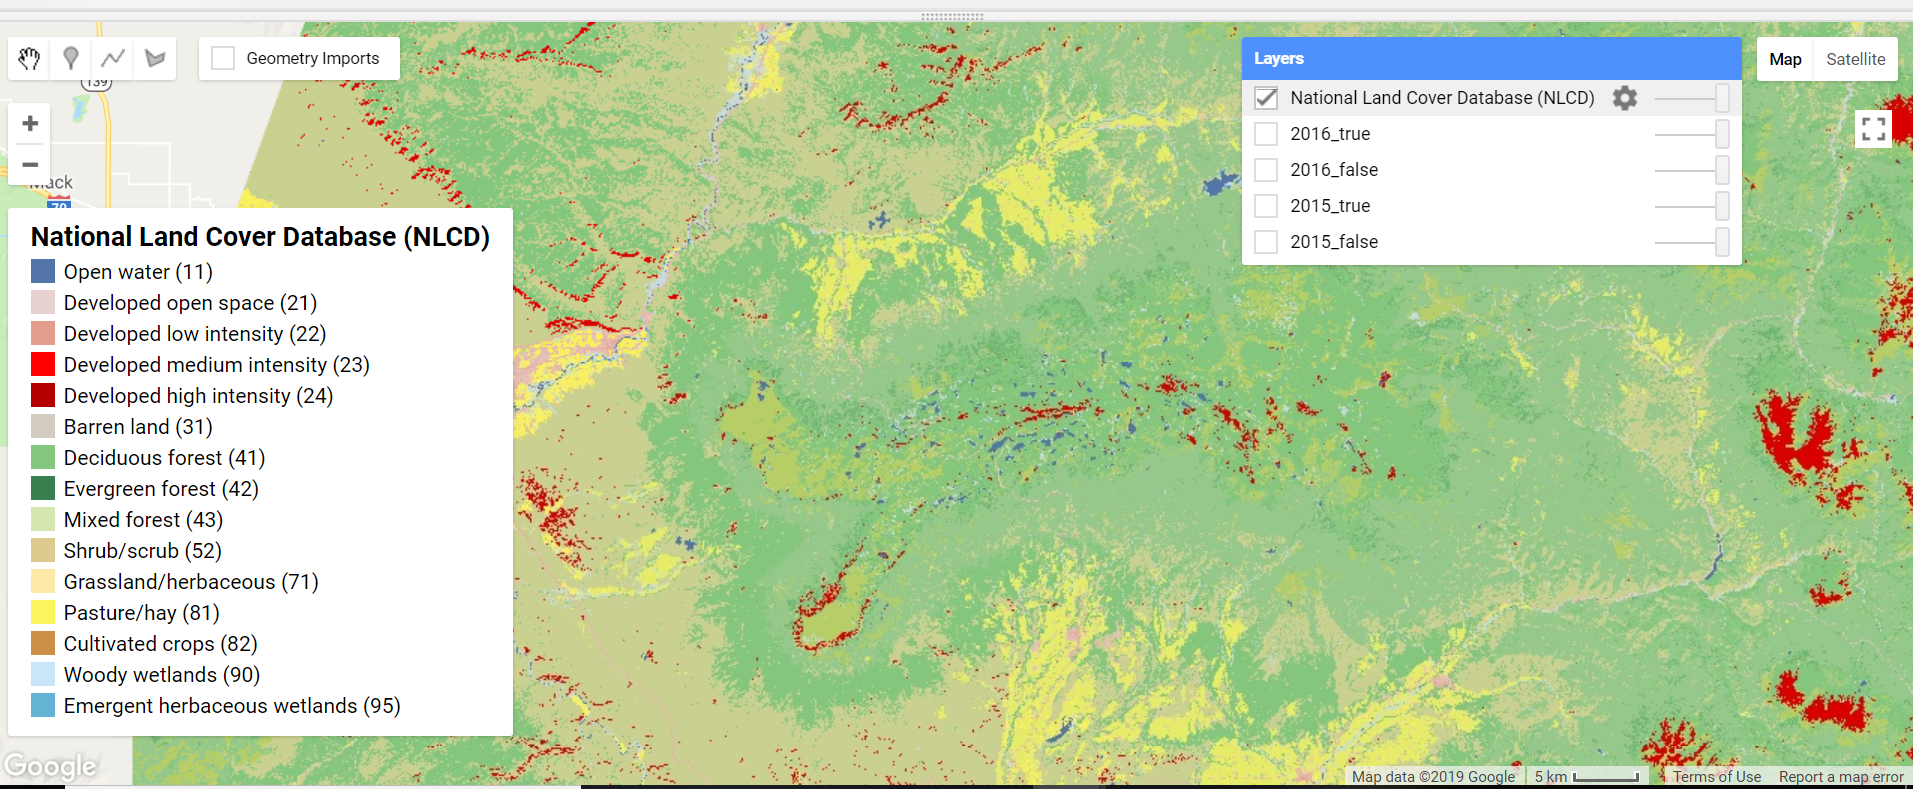
\includegraphics{Legend_NLCD_ScreenShot.png}
\caption{Legend}
\end{figure}

\subsection{Adding Presence and Absence
Locations}\label{adding-presence-and-absence-locations}

Adding in presence and absence layers is a rather straightforward
process done by creating a geometry features and placing them on
representative locations on the map.

\begin{itemize}
\item
  Let's select the import geometry box and click create new.
\item
  A geometry feature should be added below your geometry feature that is
  functioning as your area of interest.
\item
  Select the gear icon next to the text.
\item
  A pop up will open. Change the `import as' type to `FeatureCollection'
  and then press the `add Property button'
\item
  Fill in the boxes with `presence' \textbar{} 1 - change the
  featurecollection name to presence and select a color you enjoy.
  Repeat this process, creating a absence featurecollection where the
  add property looks as follows `presence' \textbar{} 0
\end{itemize}

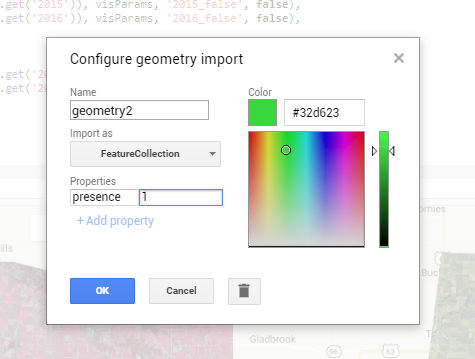
\includegraphics{presencePoints.png}

Once the points are created we can sample by selecting the specific
feature collection (presence or absence) and use the marker tool to drop
points on the imagery. The sampling methodologies you use will depend on
your study. In this example green presence points represent Aspen and
red point are not deciduous forest (absence).

 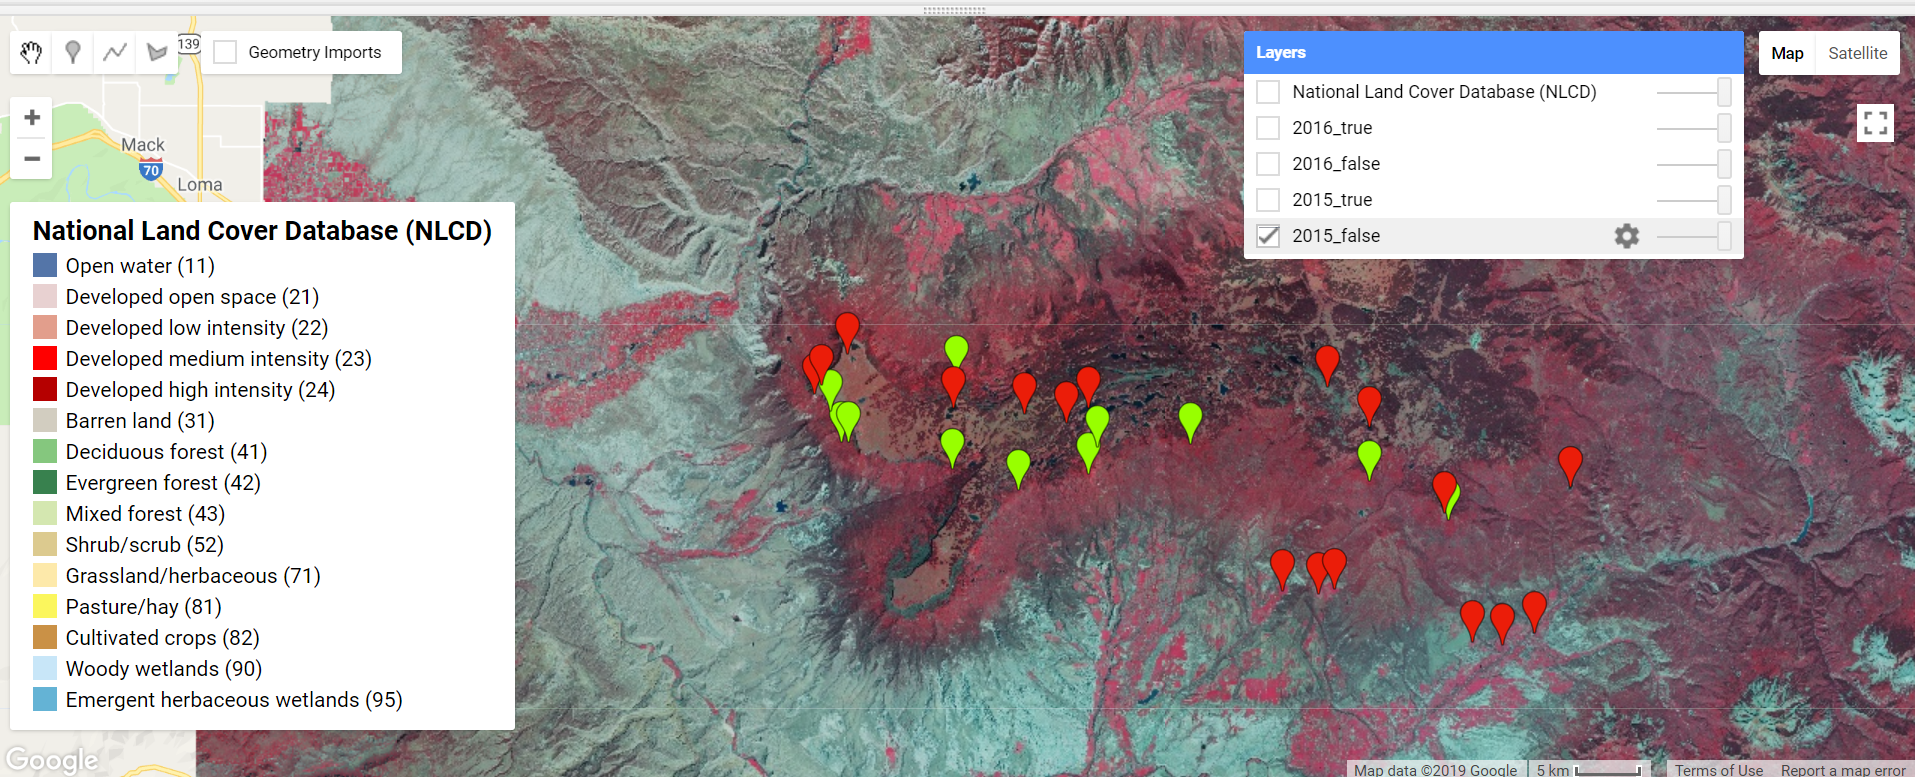
\includegraphics{Sampling_False_Color.png}

Above is a False color image Below is a NLCD image

\begin{figure}
\centering
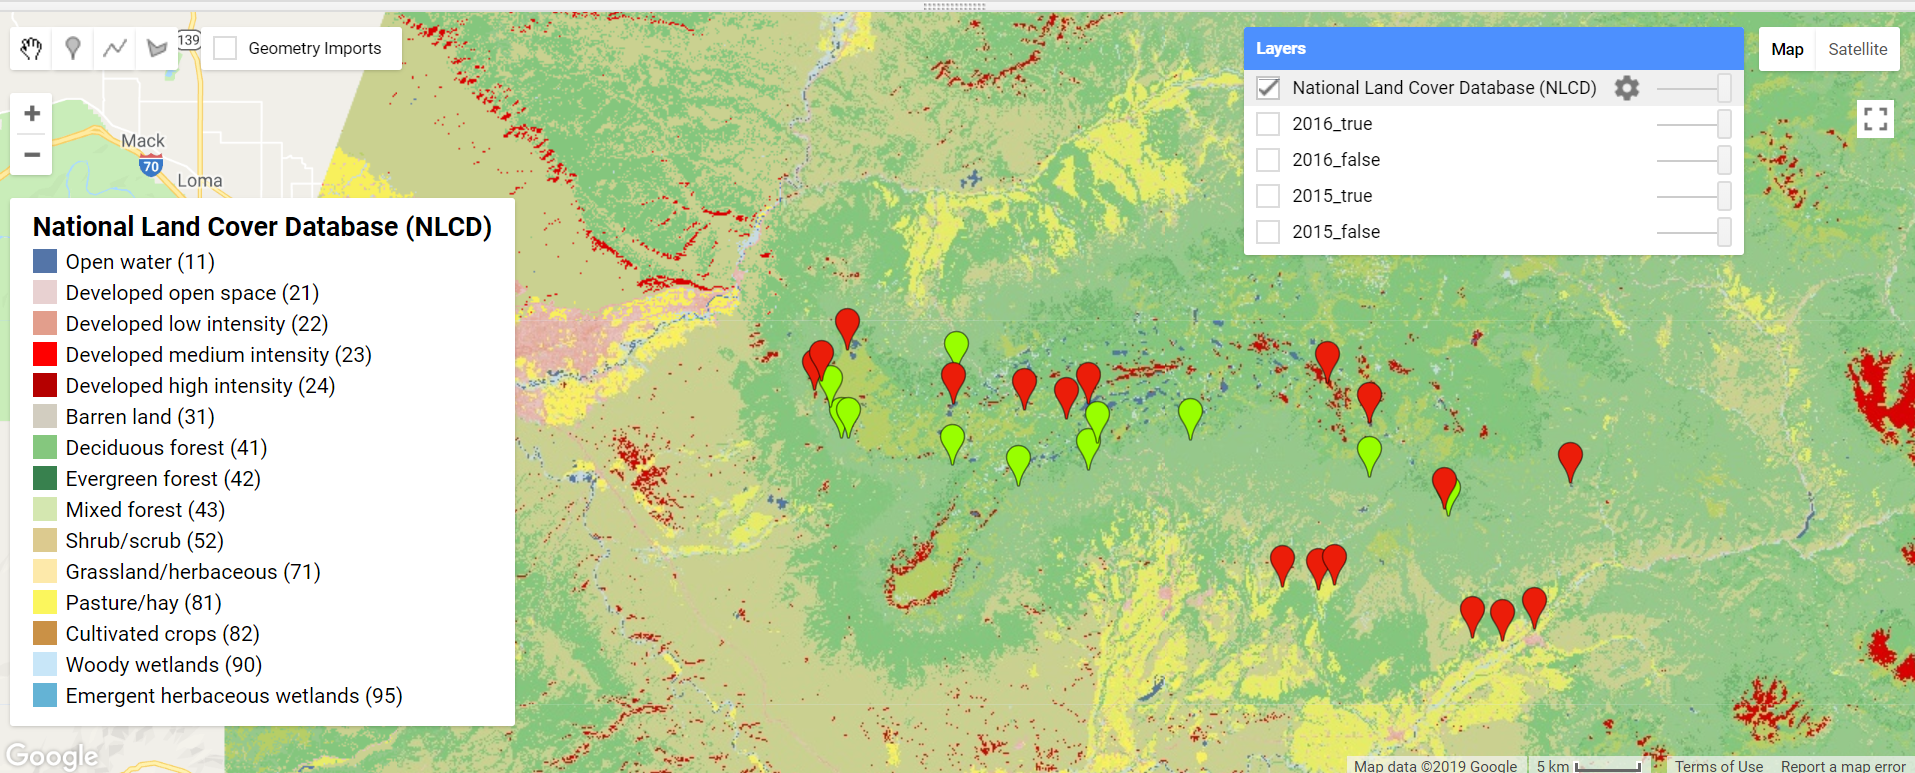
\includegraphics{Sampling_NLCD.png}
\caption{sampling example NLCD}
\end{figure}

To explore the NLCD layer when sampling, use the Inspector tool in the
console. When using the Inspector tool and clicking on the map, it will
return the class value in the console. This function is very useful for
future work with Google Earth Engine.

\begin{figure}
\centering
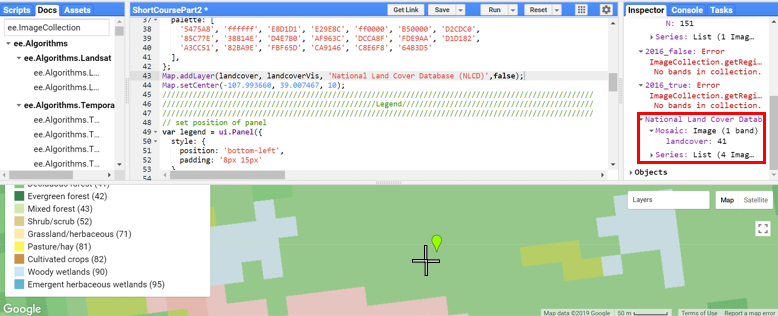
\includegraphics{Inspector_Tool.png}
\caption{Inspector Tool}
\end{figure}

\subsection{Exporting points}\label{exporting-points}

Currently our point locations are store in two different features
classes. Let's merge these features before we export the data so we are
only working with a single file.

\begin{verbatim}
//Merge presence and absence datasets
var samples = presence.merge(absence)
print(samples, 'Samples');
\end{verbatim}

Now that the sampling features classes are merged lets export the
features to the our drive. When you run the code the ``Task'' bar in the
upper right hand side of the console will light up. Google Earth Engine
does not run tasks without you specifically directing it to execute,
from the task bar.

\begin{Shaded}
\begin{Highlighting}[]
\CommentTok{//export presence points}
\VariableTok{Export}\NormalTok{.}\VariableTok{table}\NormalTok{.}\AttributeTok{toDrive}\NormalTok{(}\OperatorTok{\{}
  \DataTypeTok{collection}\OperatorTok{:}\NormalTok{ samples}\OperatorTok{,}
  \DataTypeTok{description}\OperatorTok{:}\StringTok{'presenceAbsencePointsForForest'}\OperatorTok{,}
  \DataTypeTok{fileFormat}\OperatorTok{:} \StringTok{'csv'}
\OperatorTok{\}}\NormalTok{)}
\end{Highlighting}
\end{Shaded}

 Moving material in and out of GEE can be a real challenge. While this
does produce a csv it is still take some time and effort to make match
the format you might be expecting. The best advice I have to to work
with the data in GEE for as long as you can before exporting.

\begin{figure}
\centering
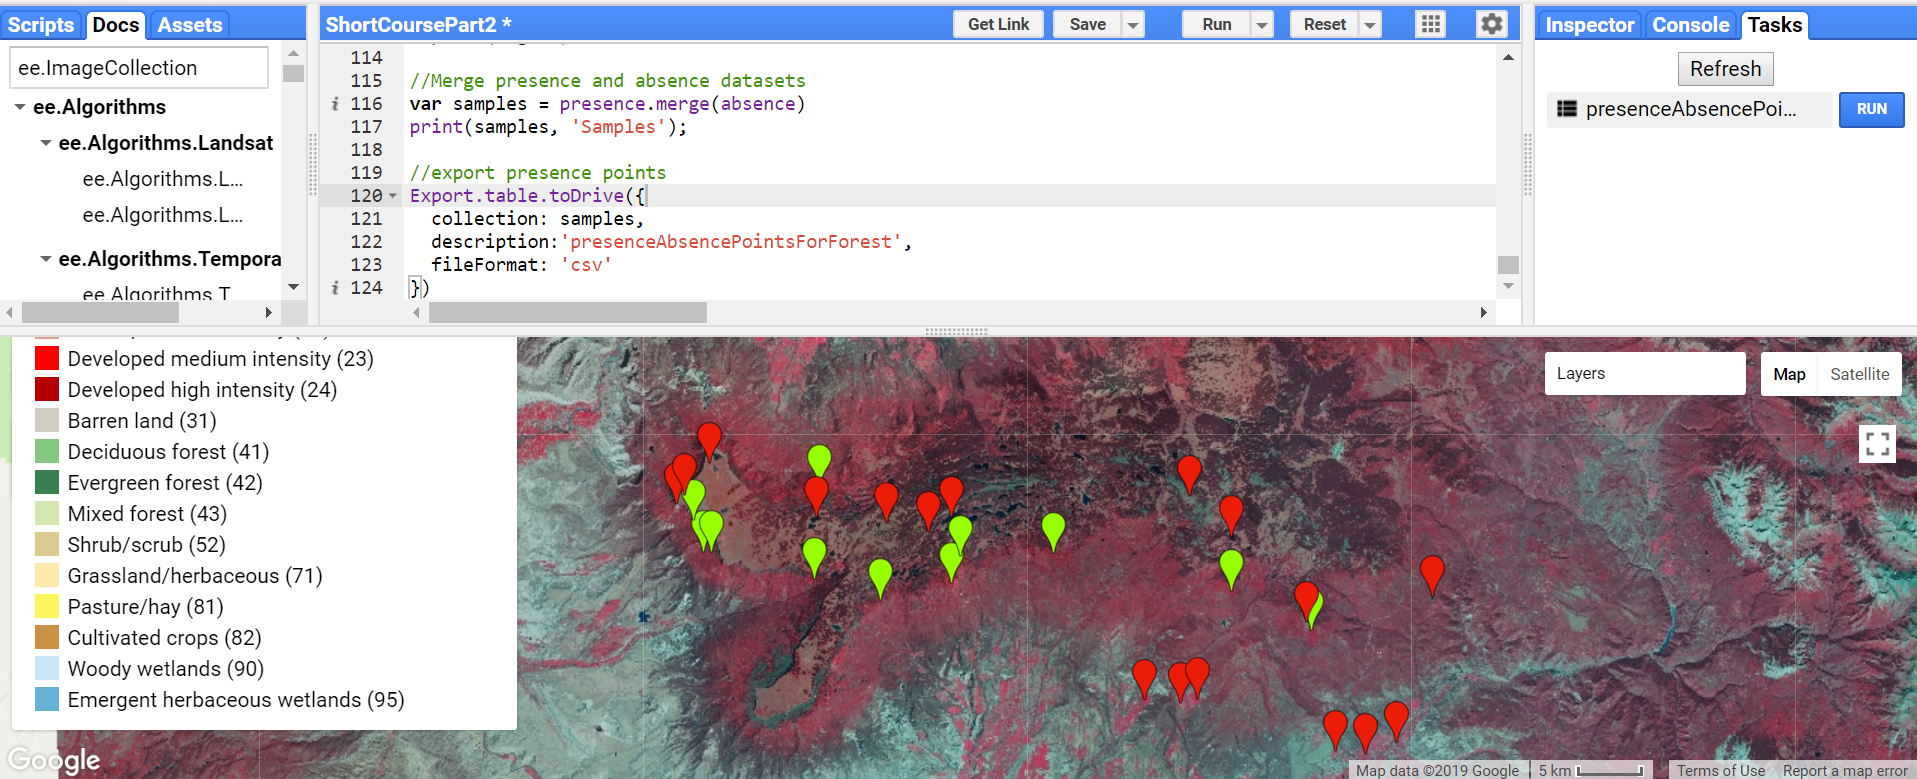
\includegraphics{Export_presence_absence_data2.png}
\caption{Export}
\end{figure}

Above is a screen capture of the exporting process Below is the final
step int he file type selection process

\begin{figure}
\centering
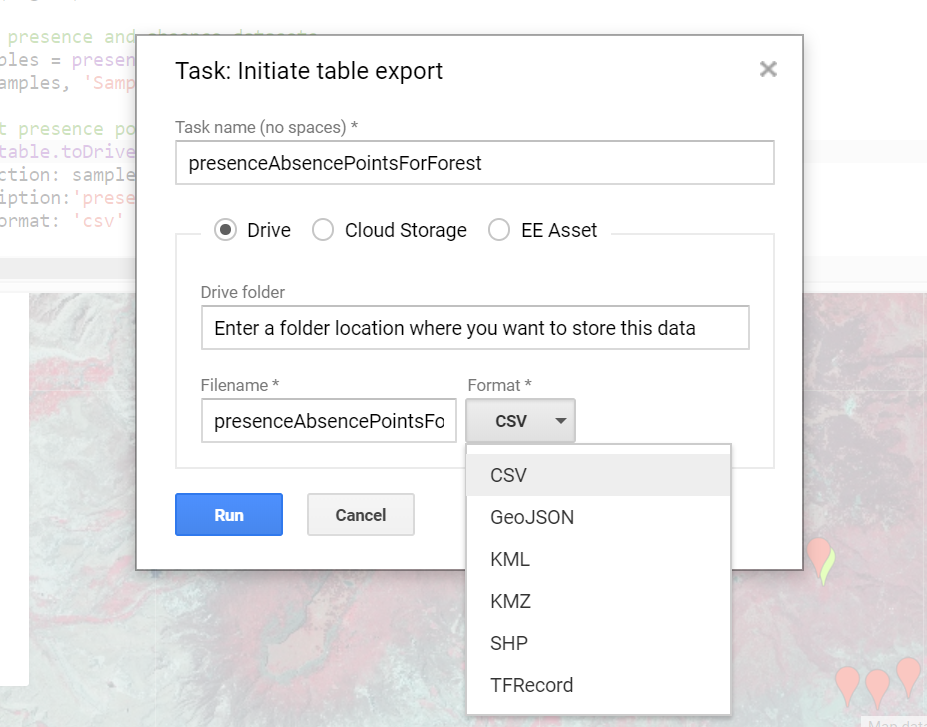
\includegraphics{File_type.png}
\caption{File Type}
\end{figure}

\subsection{Final complete code for the
lesson}\label{final-complete-code-for-the-lesson}

\begin{verbatim}
//Merge presence and absence datasets
var samples = presence.merge(absence)
print(samples, 'Samples');
\end{verbatim}

Now that the sampling features classes are merged lets export the
features to the our drive. When you run the code the ``Task'' bar in the
upper right hand side of the console will light up. Google Earth Engine
does not run tasks without you specifically directing it to execute,
from the task bar.

\begin{Shaded}
\begin{Highlighting}[]
\CommentTok{// call in NAIP imagery as an image collection }
\KeywordTok{var}\NormalTok{ NAIP }\OperatorTok{=} \VariableTok{ee}\NormalTok{.}\AttributeTok{ImageCollection}\NormalTok{(}\StringTok{"USDA/NAIP/DOQQ"}\NormalTok{)}

\CommentTok{//define viewing parameters for multi band images }
\KeywordTok{var}\NormalTok{ visParams }\OperatorTok{=} \OperatorTok{\{}\DataTypeTok{bands}\OperatorTok{:}\NormalTok{[}\StringTok{'N'}\OperatorTok{,} \StringTok{'R'}\OperatorTok{,} \StringTok{'G'}\NormalTok{]}\OperatorTok{\}}
\KeywordTok{var}\NormalTok{ visParams1 }\OperatorTok{=} \OperatorTok{\{}\DataTypeTok{bands}\OperatorTok{:}\NormalTok{[}\StringTok{'R'}\OperatorTok{,} \StringTok{'G'}\OperatorTok{,} \StringTok{'B'}\NormalTok{]}\OperatorTok{\}}


\CommentTok{// filter the data based on date and area for 2015 and 2016 }
\KeywordTok{var}\NormalTok{ naip2015 }\OperatorTok{=}\NormalTok{ NAIP}
\NormalTok{  .}\AttributeTok{filterBounds}\NormalTok{(geometry)}
\NormalTok{  .}\AttributeTok{filterDate}\NormalTok{(}\StringTok{"2015-01-01"}\OperatorTok{,} \StringTok{"2015-12-31"}\NormalTok{)}

\KeywordTok{var}\NormalTok{ naip2016 }\OperatorTok{=}\NormalTok{ NAIP}
\NormalTok{  .}\AttributeTok{filterBounds}\NormalTok{(geometry)}
\NormalTok{  .}\AttributeTok{filterDate}\NormalTok{(}\StringTok{"2016-01-01"}\OperatorTok{,} \StringTok{"2016-12-31"}\NormalTok{)}
  

\CommentTok{// add 2015 imagery to the map with false color and true color composites}
\VariableTok{Map}\NormalTok{.}\AttributeTok{addLayer}\NormalTok{(naip2015}\OperatorTok{,}\NormalTok{visParams}\OperatorTok{,}\StringTok{"2015_false"}\OperatorTok{,}\KeywordTok{false}\NormalTok{ )}
\VariableTok{Map}\NormalTok{.}\AttributeTok{addLayer}\NormalTok{(naip2015}\OperatorTok{,}\NormalTok{visParams1}\OperatorTok{,}\StringTok{"2015_true"}\OperatorTok{,}\KeywordTok{false}\NormalTok{ )}

\CommentTok{// add 2016 imagery to the map with false color and true color composites}
\VariableTok{Map}\NormalTok{.}\AttributeTok{addLayer}\NormalTok{(naip2016}\OperatorTok{,}\NormalTok{visParams}\OperatorTok{,}\StringTok{"2016_false"}\OperatorTok{,}\KeywordTok{false}\NormalTok{ )}
\VariableTok{Map}\NormalTok{.}\AttributeTok{addLayer}\NormalTok{(naip2016}\OperatorTok{,}\NormalTok{visParams1}\OperatorTok{,}\StringTok{"2016_true"}\OperatorTok{,}\KeywordTok{false}\NormalTok{ )}

\CommentTok{//add National Land Cover Database (NLCD) with color palette}
\KeywordTok{var}\NormalTok{ dataset }\OperatorTok{=} \VariableTok{ee}\NormalTok{.}\AttributeTok{ImageCollection}\NormalTok{(}\StringTok{'USGS/NLCD'}\NormalTok{)}
\CommentTok{////////comment out this line of code to unclip the NLCD layer from the geometry//////////}
\NormalTok{  .}\AttributeTok{map}\NormalTok{(}\KeywordTok{function}\NormalTok{(image) }\OperatorTok{\{} \ControlFlowTok{return} \VariableTok{image}\NormalTok{.}\AttributeTok{clip}\NormalTok{(geometry)}\OperatorTok{;} \OperatorTok{\}}\NormalTok{)}\OperatorTok{;}
\CommentTok{//}
\KeywordTok{var}\NormalTok{ landcover }\OperatorTok{=} \VariableTok{dataset}\NormalTok{.}\AttributeTok{select}\NormalTok{(}\StringTok{'landcover'}\NormalTok{)}
\CommentTok{//}
\KeywordTok{var}\NormalTok{ landcoverVis }\OperatorTok{=} \OperatorTok{\{}
  \DataTypeTok{min}\OperatorTok{:} \FloatTok{11.0}\OperatorTok{,}
  \DataTypeTok{max}\OperatorTok{:} \FloatTok{95.0}\OperatorTok{,}
  \DataTypeTok{palette}\OperatorTok{:}\NormalTok{ [}
    \StringTok{'5475A8'}\OperatorTok{,} \StringTok{'ffffff'}\OperatorTok{,} \StringTok{'E8D1D1'}\OperatorTok{,} \StringTok{'E29E8C'}\OperatorTok{,} \StringTok{'ff0000'}\OperatorTok{,} \StringTok{'B50000'}\OperatorTok{,} \StringTok{'D2CDC0'}\OperatorTok{,}
    \StringTok{'85C77E'}\OperatorTok{,} \StringTok{'38814E'}\OperatorTok{,} \StringTok{'D4E7B0'}\OperatorTok{,} \StringTok{'AF963C'}\OperatorTok{,} \StringTok{'DCCA8F'}\OperatorTok{,} \StringTok{'FDE9AA'}\OperatorTok{,} \StringTok{'D1D182'}\OperatorTok{,}
    \StringTok{'A3CC51'}\OperatorTok{,} \StringTok{'82BA9E'}\OperatorTok{,} \StringTok{'FBF65D'}\OperatorTok{,} \StringTok{'CA9146'}\OperatorTok{,} \StringTok{'C8E6F8'}\OperatorTok{,} \StringTok{'64B3D5'}
\NormalTok{  ]}\OperatorTok{,}
\OperatorTok{\};}
\VariableTok{Map}\NormalTok{.}\AttributeTok{addLayer}\NormalTok{(landcover}\OperatorTok{,}\NormalTok{ landcoverVis}\OperatorTok{,} \StringTok{'National Land Cover Database (NLCD)'}\OperatorTok{,}\KeywordTok{false}\NormalTok{)}\OperatorTok{;}
\VariableTok{Map}\NormalTok{.}\AttributeTok{setCenter}\NormalTok{(}\OperatorTok{-}\FloatTok{107.993660}\OperatorTok{,} \FloatTok{39.007467}\OperatorTok{,} \DecValTok{10}\NormalTok{)}\OperatorTok{;}
\CommentTok{///////////////////////////////////////////////////////////////////////////////////////////////////}
\CommentTok{/////////////////////////////////////////////////Legend////////////////////////////////////////////}
\CommentTok{///////////////////////////////////////////////////////////////////////////////////////////////////}
\CommentTok{// set position of panel}
\KeywordTok{var}\NormalTok{ legend }\OperatorTok{=} \VariableTok{ui}\NormalTok{.}\AttributeTok{Panel}\NormalTok{(}\OperatorTok{\{}
  \DataTypeTok{style}\OperatorTok{:} \OperatorTok{\{}
    \DataTypeTok{position}\OperatorTok{:} \StringTok{'bottom-left'}\OperatorTok{,}
    \DataTypeTok{padding}\OperatorTok{:} \StringTok{'8px 15px'}
  \OperatorTok{\}}
\OperatorTok{\}}\NormalTok{)}\OperatorTok{;}

\CommentTok{// Create legend title}
\KeywordTok{var}\NormalTok{ legendTitle }\OperatorTok{=} \VariableTok{ui}\NormalTok{.}\AttributeTok{Label}\NormalTok{(}\OperatorTok{\{}
  \DataTypeTok{value}\OperatorTok{:} \StringTok{'National Land Cover Database (NLCD)'}\OperatorTok{,}
  \DataTypeTok{style}\OperatorTok{:} \OperatorTok{\{}
    \DataTypeTok{fontWeight}\OperatorTok{:} \StringTok{'bold'}\OperatorTok{,}
    \DataTypeTok{fontSize}\OperatorTok{:} \StringTok{'18px'}\OperatorTok{,}
    \DataTypeTok{margin}\OperatorTok{:} \StringTok{'0 0 4px 0'}\OperatorTok{,}
    \DataTypeTok{padding}\OperatorTok{:} \StringTok{'0'}
    \OperatorTok{\}}
\OperatorTok{\}}\NormalTok{)}\OperatorTok{;}

\CommentTok{// Add the title to the panel}
\VariableTok{legend}\NormalTok{.}\AttributeTok{add}\NormalTok{(legendTitle)}\OperatorTok{;}
    
\CommentTok{// Creates and styles 1 row of the legend.}
\KeywordTok{var}\NormalTok{ makeRow }\OperatorTok{=} \KeywordTok{function}\NormalTok{(color}\OperatorTok{,}\NormalTok{ name) }\OperatorTok{\{}
      
      \CommentTok{// Create the label that is actually the colored box.}
      \KeywordTok{var}\NormalTok{ colorBox }\OperatorTok{=} \VariableTok{ui}\NormalTok{.}\AttributeTok{Label}\NormalTok{(}\OperatorTok{\{}
        \DataTypeTok{style}\OperatorTok{:} \OperatorTok{\{}
          \DataTypeTok{backgroundColor}\OperatorTok{:} \StringTok{'#'} \OperatorTok{+}\NormalTok{ color}\OperatorTok{,}
          \CommentTok{// Use padding to give the box height and width.}
          \DataTypeTok{padding}\OperatorTok{:} \StringTok{'8px'}\OperatorTok{,}
          \DataTypeTok{margin}\OperatorTok{:} \StringTok{'0 0 4px 0'}
        \OperatorTok{\}}
      \OperatorTok{\}}\NormalTok{)}\OperatorTok{;}
      
      \CommentTok{// Create the label filled with the description text.}
      \KeywordTok{var}\NormalTok{ description }\OperatorTok{=} \VariableTok{ui}\NormalTok{.}\AttributeTok{Label}\NormalTok{(}\OperatorTok{\{}
        \DataTypeTok{value}\OperatorTok{:}\NormalTok{ name}\OperatorTok{,}
        \DataTypeTok{style}\OperatorTok{:} \OperatorTok{\{}\DataTypeTok{margin}\OperatorTok{:} \StringTok{'0 0 4px 6px'}\OperatorTok{\}}
      \OperatorTok{\}}\NormalTok{)}\OperatorTok{;}
      
      \CommentTok{// return the panel}
      \ControlFlowTok{return} \VariableTok{ui}\NormalTok{.}\AttributeTok{Panel}\NormalTok{(}\OperatorTok{\{}
        \DataTypeTok{widgets}\OperatorTok{:}\NormalTok{ [colorBox}\OperatorTok{,}\NormalTok{ description]}\OperatorTok{,}
        \DataTypeTok{layout}\OperatorTok{:} \VariableTok{ui}\NormalTok{.}\VariableTok{Panel}\NormalTok{.}\VariableTok{Layout}\NormalTok{.}\AttributeTok{Flow}\NormalTok{(}\StringTok{'horizontal'}\NormalTok{)}
      \OperatorTok{\}}\NormalTok{)}\OperatorTok{;}
\OperatorTok{\};}


\CommentTok{//  Palette with the colors}
\KeywordTok{var}\NormalTok{ palette }\OperatorTok{=}\NormalTok{[}\StringTok{'5475A8'}\OperatorTok{,}\StringTok{'E8D1D1'}\OperatorTok{,}\StringTok{'E29E8C'}\OperatorTok{,}\StringTok{'ff0000'}\OperatorTok{,}\StringTok{'B50000'}\OperatorTok{,}\StringTok{'D2CDC0'}\OperatorTok{,}\StringTok{'85C77E'}\OperatorTok{,}\StringTok{'38814E'}\OperatorTok{,}\StringTok{'D4E7B0'}\OperatorTok{,}
\StringTok{'DCCA8F'}\OperatorTok{,}\StringTok{'FDE9AA'}\OperatorTok{,}\StringTok{'FBF65D'}\OperatorTok{,}\StringTok{'CA9146'}\OperatorTok{,}\StringTok{'C8E6F8'}\OperatorTok{,}\StringTok{'64B3D5'}\NormalTok{]}\OperatorTok{;}
    

\CommentTok{// name of the legend}
\KeywordTok{var}\NormalTok{ names }\OperatorTok{=}\NormalTok{ [}
\StringTok{'Open water (11)'}\OperatorTok{,} \StringTok{'Developed open space (21)'}\OperatorTok{,}\StringTok{'Developed low intensity (22)'}\OperatorTok{,}\StringTok{'Developed medium intensity (23)'}\OperatorTok{,}\StringTok{'Developed high intensity (24)'}\OperatorTok{,} \StringTok{'Barren land (31)'}\OperatorTok{,} \StringTok{'Deciduous forest (41)'}\OperatorTok{,}\StringTok{'Evergreen forest (42)'}\OperatorTok{,}\StringTok{'Mixed forest (43)'}\OperatorTok{,}\StringTok{'Shrub/scrub (52)'}\OperatorTok{,}\StringTok{'Grassland/herbaceous (71)'}\OperatorTok{,}\StringTok{'Pasture/hay (81)'}\OperatorTok{,}\StringTok{'Cultivated crops (82)'}\OperatorTok{,}\StringTok{'Woody wetlands (90)'}\OperatorTok{,} \StringTok{'Emergent herbaceous wetlands (95)'}
\NormalTok{]}\OperatorTok{;}

\CommentTok{// Add color and and names}
\ControlFlowTok{for}\NormalTok{ (}\KeywordTok{var}\NormalTok{ i }\OperatorTok{=} \DecValTok{0}\OperatorTok{;}\NormalTok{ i }\OperatorTok{<} \VariableTok{names}\NormalTok{.}\AttributeTok{length}\OperatorTok{;}\NormalTok{ i}\OperatorTok{++}\NormalTok{) }\OperatorTok{\{}
  \VariableTok{legend}\NormalTok{.}\AttributeTok{add}\NormalTok{(}\AttributeTok{makeRow}\NormalTok{(palette[i]}\OperatorTok{,}\NormalTok{ names[i]))}\OperatorTok{;}
  \OperatorTok{\}}  

\CommentTok{// add legend to map (alternatively you can also print the legend to the console)  }
\VariableTok{Map}\NormalTok{.}\AttributeTok{add}\NormalTok{(legend)}\OperatorTok{;}  

\CommentTok{//Merge presence and absence datasets}
\KeywordTok{var}\NormalTok{ samples }\OperatorTok{=} \VariableTok{presence}\NormalTok{.}\AttributeTok{merge}\NormalTok{(absence)}
\AttributeTok{print}\NormalTok{(samples}\OperatorTok{,} \StringTok{'Samples'}\NormalTok{)}\OperatorTok{;}

\CommentTok{//export presence points}
\VariableTok{Export}\NormalTok{.}\VariableTok{table}\NormalTok{.}\AttributeTok{toDrive}\NormalTok{(}\OperatorTok{\{}
  \DataTypeTok{collection}\OperatorTok{:}\NormalTok{ samples}\OperatorTok{,}
  \DataTypeTok{description}\OperatorTok{:}\StringTok{'presenceAbsencePointsForForest'}\OperatorTok{,}
  \DataTypeTok{fileFormat}\OperatorTok{:} \StringTok{'csv'}
\OperatorTok{\}}\NormalTok{)}
\CommentTok{///End of code///}
\end{Highlighting}
\end{Shaded}


\end{document}
